\chapter{Change detection for RTT measurements}
\label{sec:cpt_rtt}

\section*{Abstract}
There are two major motivations for the study on change detection for \ac{RTT} measurements, both of which contributes to measurement-based intradomain \ac{TE}.
First, moments of important changes in RTT measurements can serve as trigger for route re-selection, focus of current chapter.
Second, it helps describe synchronized RTT observed in chapter~\ref{sec:infer}.

%In section XX, we further discuss how change detection is employed in inferring the causes of RTT changes, which eventually provide clue to TE decisions for destination prefixes with out hosts that can be probed.

Change detection methods, conceived for the robust yet relevant detection of significant change in time series, is a competent tool for RTT measurement processing.
Among the extensive works on change detection methods and their applications in various domains, few focus on RTT measurements. It is thus unclear which approach works the best on such data.  
In this chapter, we present an evaluation framework for change detection on RTT times series, consisting of:
\begin{enumerate}
	\item a carefully labelled 34,008-hour RTT dataset as ground truth;
	\item a scoring method specifically tailored for RTT measurements.
Furthermore, we proposed a data transformation that improves the detection performance of existing methods.
\end{enumerate}

In the purpose of discussing change detection sensitivity and relevance with regard to network events, path changes are as well attended to. 
We fix shortcomings of previous works by distinguishing path changes due to routing protocols (IGP and BGP) from those caused by load balancing. 
We apply our change detection methods to a large set of measurements from RIPE Atlas. 
The characteristics of both RTT and path changes are analyzed; the correlation between the two are also illustrated. 
\clearpage


\section{RTT changes: the trigger for interdomain TE}
RTT measurements intervene in measurement-based interdomain TE at two phases. 
First, RTT measurements reveals the moments when route re-selection is needed, otherwise the transmission performance may undergo avoidable degradation.  
Second, RTT measurements serve as decision making material in route re-selection. We relay on the measured delay, transmission cost and routing politics and etc., to decide which path/transit provider is the best choice  in reaching a each destination at certain moment. 
We focus on the first phase in this chapter.

Moments when route re-selection is needed are basically when significant changes happen in certain RTT measurements. In order to detect changes in numerous RTT time series of different characteristics stemmed from various underlying Internet paths, the detection method should 1) be capable of tolerating noises in RTT measurements, such as short living spikes, yet remain sensitive to events that really matter; 2) be free of ad hoc, e.g. destination dependent, parameters in achieving the desired robustness. 
Change detection methods, fitted candidate for such task, aim exactly at detecting moments of changes that cut time series into segment of different statistic characteristics.

Before studying how change detection methods work on RTT time series, we first look at some straightforward way of employing RTT measurements in TE. We explain why these possible practices are not good enough and hence justify our study on change detection methods.

\marginpar{Some straw-man practices. Other possibilities may as well work.}
\paragraph{Preference over smaller average RTT} Continuously repeated RTT measurements over time can tell which transit provider among available ones offers the smallest delay in average in reaching a specific destination. Employing this transit provider can thus ensure a good overall performance. However, this approach falls short in handling transient RTT augmentation during for example congestion.

\paragraph{Threshold of RTT value} In order to mitigate the consequence of stiff route choice, one can introduce some dynamism by simply comparing the instant RTT measurements with a hard-coded threshold. Once the RTT surpasses the threshold value, even through the transit with smallest average RTT, route re-selection can be trigger to look for a better performance path at that specific moment.
The drawback of this method is that the threshold values depend on each individual destination, and are thus not trivial to configure.

\paragraph{Threshold of RTT change amplitude} Focusing on the difference of consecutive measurements in time rather than the instant RTT value can transform the ad hoc RTT value threshold to a change amplitude threshold reused by all destinations. \marginpar{Here RTT change refers to the value difference between two RTT measurements. Elsewhere, RTT change means the change in RTT time series detected by change detection methods.}
This change amplitude threshold could be absolute values such as 30 msec or a percentage, e.g. $30\%$,  making the change amplitude in msec proportionally adapted to the level of RTT.
The shortcoming of this approach comes from the fact that RTT measurements (via ICMP or TCP) could be pretty noisy, full of shorting living yet large amplitude variations, leading to unnecessarily frequent route re-selection.

\paragraph{Smoothing the RTT measurements} One straightforward to remain robust when handling noisy RTT measurement is to smooth it before usage. A possible way is the perform \ac{EWMA} over a couple of past measurements~\cite{Akella2008}. However, the application of such filters introduces additional parameters to be tuned, and likely in an ad hoc manner. Moreover, such filter will as well introduce a delay to the perception of an actual change.


\section{RTT change, network events and TE}
\label{sec:rtt_path}
In this section, we summarize previous studies on RTT variations and the network events that causes RTT changes.
We explain why certain RTT analysis method adopted in mentioned works is not a good fit for TE uses.

Path changes and congestion are known to be the major reasons for RTT changes.
It is generally agreed that inter-domain routing changes impact the RTT level greatly.
Pucha et al.~\cite{Pucha2007} showed that inter-domain routing changes cause larger median RTT variation than intra-domain ones.
Rimondini et al.~\cite{Rimondini2014} confirmed that $72.5\%$ BGP route changes in their study are associated with RTT change.
%% Measurement from RIPE Atlas and RIPE RIS back in 2013, only 55 AS is considered.
Similar observations were made in a large \ac{CDN}, where inter-domain routing changes are responsible for more than $40\%$ of severe user experience degradation~\cite{Zhu2012}.

Intra-domain events are no less important. Pucha et al.~\cite{Pucha2007} discovered that intra-domain path changes can cause RTT changes of comparable amplitude as inter-domain ones.
Moreover, they pointed out that it is intra-domain path changes, not congestion, that are responsible for the majority ($86\%$) of RTT changes. %instead of congestion.
A different claim was however made by Schwartz et al.~\cite{Schwartz2010}. They found out that most RTT variation is rather within paths (i.e. due to congestion) than among paths (i.e. due to path changes).

Conflicts in previous works could be caused by the difference in locations from where measurements were launched.
For instance, Chandrasekaran et al.~\cite{Chandrasekaran} observed that AS path changes only have marginal impact on RTT in the core of Internet, while previous works~\cite{Pucha2007, Schwartz2010} include as well access networks.
Results might as well change over time. For instance, the ``flattened'' Internet topology, the increasing amount of traffic in private CDN over the last decade~\cite{Labovitz2011, Roughan2011} might have changed the characteristics of path change and congestion, and consequently how they impact RTT.

Bearing this in mind, we emphasize the efforts on methods and tools enabling iterative
analysis on the relationship between RTT and path changes over time, rather than one shot observation or analysis on a specific dataset.

The discussion and discovery of previous works are enlightening, yet their methods of processing RTT measurements can hardly fuel RTT change triggered intra-domain TE.
In ~\cite{Pucha2007, Schwartz2010, Chandrasekaran},
RTT measurements are first grouped by underlying paths; impact of path changes are then estimated through comparison of associated RTT statistics, e.g. percentiles.
In our TE scheme, RTT rather than path are more intensively measured~\cite{shao2016}.
This is because path measurements do not necessarily reflect all the changes in RTT, meanwhile being more resource-consuming.
For example, congestion in upstream network can only be learnt through change detection on RTT measurements.

\section{Code space and data}
\label{sec:cpt_data}
%%% Why is it part of the "Related Work" section ? 
%%% Wenqin: it is not. The related work section remains to be filled.
The main code space for work in this chapter is made public on Github with documentation: \url{https://github.com/WenqinSHAO/rtt}.
The implementations of proposed methods are decoupled from the context of this project, and thus can easily be employed elsewhere.  

We applied our methods on RIPE Atlas built-in measurements~\cite{atlas} and performed data analysis.
These measurements are openly available so that the results of this work can be reproduced by other researchers or compared to alternative approaches.
We collected RIPE Atlas built-in ping and traceroute measurement toward DNS b-root (measurement ID 1010, 5010) from 6029 v3 probes located in 2050 different ASes, 153 countries from 2016-10-01 to 2017-01-01~\footnote{Measurements to other destinations might as well do. The fact whether the destination is anycast or not is of few importance in this work. The focus is on method rather than on a specific dataset.}.
184,358,516 ping and 23,507,910 traceroute measurements are collected and analyzed.
The traceroute measurements flowed through 3036 ASes, 120 IXPs, containing 10720 different AS paths.
%The script and the configurations to collect above data are as well included in the project repository.


\section{Changepoint detection}
\label{sec:cpt}
In this section, we introduce change detection method and its previous application on RTT measurements.

% Such changes are generally caused by path change or congestion, and thus have important implications in networking and traffic engineering.
\subsection{A primer on change detection}
The moments that cut a time series into segments of different characteristics are called \textit{changepoints}.
The problem of detecting the most appropriated changepoints is known as changepoint detection or change detection.

One common approach to changepoint detection translates the quest of finding the best changepoints into the following optimization problem \footnote{Other formulations exist. A wider literature can be found in \cite{Haynes2016, Eckley2011}. We focus on this approach in this work since it has well maintained libraries that prevent potential issues regarding the implementation~\cite{Killick2013a, Haynes2016}.}.
Assume we are given a sequence of data, $y_{1:n} = (y_1, y_2,...y_n)$.
We expect changepoint detection method to produce $m$ ordered changepoints, $\tau_{1:m} = (\tau_1, \tau_2,...\tau_m)$.
$\tau_i$ is the position of $i^{th}$ changepoints and takes value from in ${1,..,n-1}$.
These changepoints are given in an ordered way such that $\tau_i < \tau_j$ if and only if $i < j$.
We define $\tau_0 = 0$ and $\tau_{m+1} = n$.
Together with the detected $m$ changepoints, they cut $y_{1:n}$ into $m+1$ segments, with the $i_{th}$ segment containing $y_{\tau_{i-1}+1:\tau_i}$.
For each segment, a cost is calculated. The detection method seeks to minimize the cost sum of all the segments: 
\begin{equation}
\sum_{i=1}^{m+1}[C(y_{\tau_{i-1}:\tau_i-1})] + \beta f(m).
\end{equation}
Here $C$ is a cost function while $\beta f(m)$ is a penalty to prevent over-fitting ---  the two major parameters to be set.

One commonly used cost function is minus of the maximum log-likelihood of the segment following a certain distribution~\cite{Killick2011,Horvath1993,Chen2001}:
\begin{equation}
C(y_{s:t}) = - \max_\theta \sum_{i=s}^t \log f(y_i|\theta).
\end{equation}
Here $f(y|\theta)$ is a density function with distribution parameter $\theta$. 
For example, if we assume a Normal distribution, then we have $\theta = (\mu, \delta^2)$:
$f(y|\theta) = f(y|\mu, \delta^2) = \frac{1}{\sqrt{2\delta^2\pi}} e^{-\frac{(x-\mu)}{2\delta^2}}$.
In such case, the choice of cost function is restrained to the choice of distribution types.
Currently supported distributions in \cite{Killick2013a} are: Normal, Exponential, Gamma and Poisson.
A recent progress proposes a cost function based on empirical distribution likelihood, where the specification on distribution type is not necessary. It is thus a non-parametric method~\cite{Haynes2016}. 

When it comes to penalty, $f(m)$ is generally a function linear to the number of parameters introduced by $m$ changepoints: 
$m + (m+1)dim(\theta)$ \footnote{$dim(\theta)$ is the dimension of $\theta$. In the case of Normal distribution, $dim(\theta) = 2$.}.
%%% JLR: dim ??? Not explicit for people not familiar with these works.
%%% Wenqin: footnote added.
Common choices of $\beta$ are information criteria, such as Akaike’s Information Criterion (AIC) with $\beta=2$, Schwarz Information Criterion (SIC, also known as BIC) with $\beta=\log n$, Hannan-Quinn Information Criterion with $\beta = 2 \log \log n$, and Modified BIC (MBIC) with 
$\beta f(m) = -\frac{1}{2} [3f(m)\log n + \sum_{i=1}^{m+1} log(r_i - r_{i-1})]$, where $r_i = \tau_i/n$~cite{Zhang2007}.
We have MBIC $>$ BIC $>$ Hannan Quinn. Note that larger penalty value leads to less sensitive detection.

\subsection{Application of change detection to RTT measurements}
RTT traces, like many other time series, may undergo sudden changes in level or volatility, generally caused by path change or congestion.
Among the extensive studies on change detection methods and their applications in various domains~\cite{Zhang2007,Reeves2007, Yu2008},
Rimondini et al.~\cite{Rimondini2014} are among the first to employ change detection in network RTT measurement analysis.
However, they tuned the detection sensitivity in a way that detected changes correlate best to the BGP changes of the destination prefix among other randomly selected prefixes, which potentially ignores the RTT change due to intra-domain changes and congestion.
Plus, such tuning is potentially required for each individual RTT time series, thus hard to scale.
To achieve more general approach decoupled from path measurements, we propose in next section an evaluation framework for the selection and calibration of change detection methods for RTT measurements.


\section{Evaluation framework for changepoint detection on RTT measurements}
\label{sec:eval_frame}
Which method (among the wide variety of existing ones) is the most appropriate for Internet RTT time series is still not stated. Moreover, many changepoint detection methods are parametric. Identifying the best settings for these methods remains challenging.
One fundamental issue in addressing the above problems is the lack of an evaluation framework.

An evaluation framework should be composed of two parts: 1) datasets of ``ground truth'', 2) a scoring method.
We are not aware of any RTT time series labelled with moments of change that are publicly available as of this writing.
We manually labelled 50 real RTT time series from RIPE Atlas containing 408,087 RTT measurements.
Details are given in Sec.~\ref{sec:label}.

As for the scoring method, classic true/false positive classification is too rigid for 
both manual labelling and change point detection, see Sec.~\ref{sec:score}.
We argue that a slight shift in time could be tolerated.
% Numenta proposed an evaluation method (for anomaly detection) with window option~\cite{Lavin2016}. However, they attribute equal weight to each ground truth events of anomaly (wich are homologous to RTT changes in our case). 
We propose weighting each actual RTT changes according to their operational importance. 

\subsection{Scoring methods}
\label{sec:score}

We assume ground truth $T_{1:k}$ containing $k$ positions in $y_{1:n}$ indicating moments of actual change, while $\tau_{1:m}$ is the output of changepoint detection.
A classic True Positive ($TP$) is a $\tau_j, \exists T_i \in T_{1:k}, T_i = \tau_j$, a False Positive ($FP$) otherwise. False Negative ($FN$) composes of $\{T_i \mid \nexists \tau_j \in \tau_{1:m}, \tau_j = T_i \}$.
However, there are many times during labeling that finding a clear cut position for certain RTT changes is difficult for human beings, and the labeled moment of change might reasonably vary within a range.
It is therefore too harsh to require exact match from change detection.

Introducing a window of tolerance $w$, we are confronted with an issue where 
$T_i$ can be detected by multiple detection outputs $ \{\tau_j \mid |\tau_j - T_i| \leq w \}$. 
Symmetrically, $\tau_j$ can be associated with several $T_i$ within the tolerance window.
If many-to-many mapping between $T_{1:k}$ and $\tau_{1:m}$ is allowed, the number of $TP$ could be overestimated. while $FN$ underestimated.

One straightforward solution adopted by Numenta is that a $T_i$ can only be detected
by the closest detection in the window $\hat \tau_i$~\cite{Lavin2016}. All the rest detected changes will be ignored.
The problem with this approach is that the actual change that is closest to the above $\hat \tau_i$, denoted as $\hat T_i$, doesn't necessary satisfy $\hat T_i = T_i$. 
Such discrepancy indicates that the mapping between ground fact and detection is potentially not optimal in two aspects:
\begin{enumerate}
\item $\hat T_i$ could end up undetected even though there are detection points within the window;
\item the overall time shift between truth and detection is not necessary the minimum.
\end{enumerate}

We henceforth define an optimal mapping between $T_{i:k}$ and $\tau_{i:m}$ with shift tolerance $w$ , $MP = \{(T_x, \tau_y)\} \mid |T_x - \tau_y| \leq w \}$, as one that first maximizes $|MP|$, the size of $MP$, and then minimizes the total shift $\sum_{(T_x, \tau_y) \in MP} |T_x - \tau_y|$. 
We first construct a bipartite graph with cost $G = (V \cup W, E)$.
$V \cup W$ are the vertices, where $V = T_{i:k}$ and $W = \tau_{1:m}$.
Edge $E$ is composed of all ground truth and detected change point pairs that are within the window, $E = \{(p, q) \mid |p - q| \leq w, p \in V, q \in W \}$.
The cost of each edge is defined as the distance/shift in time between ground truth and the detected change point $C(e) = |p-q|, e \in E$.
The problem of finding the optimal mapping $MP$ is translated into finding the \textit{minimum cost maximum-cardinality matching} of $G$, for which the Hungarian algorithm is known as the best option.

For each detection $\tau_j$, if $\exists m \in MP, \tau_j \in m$, it is regarded as a $TP$, otherwise as a $FP$.
All the ground truth without matched detection $\{T_i \mid \nexists m \in MP, T_j \in m\}$ contributes to $FN$.
$Precision$ of the changepoint detection method, defined as  $\frac{TP}{TP+FP}$, can be interpreted as the fraction of detection that is relevant or useful.
$Recall$, defined as $\frac{TP}{TP+FN}$, can be regarded as the fraction of all ground truth change points that the method can successfully detect.

Each detected change may be treated equally, yet not all ground truth RTT changes are equally important. 
We propose to weight a ground truth change $T_i$ according to the following three elements:
\begin{enumerate}
\item the length of RTT segment following $T_i$, i.e. $T_{i+1} - T_i$;
\item the RTT level difference across $T_i$, denoted as $M_i$; 
\item the RTT volatility difference across $T_i$, denoted as $\Delta_i$.
\end{enumerate}
More formally for each $T_i \in T_{i:k}$, with $T_0=1, T_{k+1} = n$, we define:
\begin{equation}
M_i = |Median(y_{T_{i-1}+1:T_i}) - Median(y_{T_i+1:T_{i+1}})|.
\end{equation}
We use median instead of mean in the purpose of reducing the impact of abnormally large RTT measurements.
We define:
\begin{equation}
\Delta_i = |Std(y_{T_{i-1}+1:T_i}) - Std(y_{T_i+1:T_{i+1}})|,
\end{equation}
as the measure for variance change across the changepoint.
We define empirically the weight associated to each $T_i \in T_{1:k}$ as:
\begin{equation}
\Omega_i = MAX(\log_2\frac{T_{i+1} - T_i}{\rho}, 0) \times (M_i + \Delta_i).
\end{equation}
Here $\rho$ is a threshold for RTT segment length. 
If $T_i$ leading to an RTT segment shorter than $\rho$, we ignore it in calculating $Recall$.
The intuition behind this weighting is that RTT changes of large level or volatility are in practice regarded as more important. $\rho$ and $w$ tolerance window are set to $8min$ in this work, corresponding to two ping measurement intervals. 

We can henceforth formulate a `weighted' version of the $Recall$ metric to better reflect the operational importance of detected RTT changes: $Recall_W = \frac{\sum_{i, T_i \in TP} \Omega_i}{\sum_{j=1}^k \Omega_j}.$

We use the $F_2$ score to consolidate $precision$ and $recall$, where recall is weighted twice as important as precision: $F_2 = (1+2^2) \times \frac{Precision \times Recall}{2^2Precsion + Recall}.$
The practical implication of this choice is that handling some FPs is less unwanted than missing out some important RTT changes.

\subsection{Ground truth dataset}
\label{sec:label}

\begin{figure}[!htb]
\centering
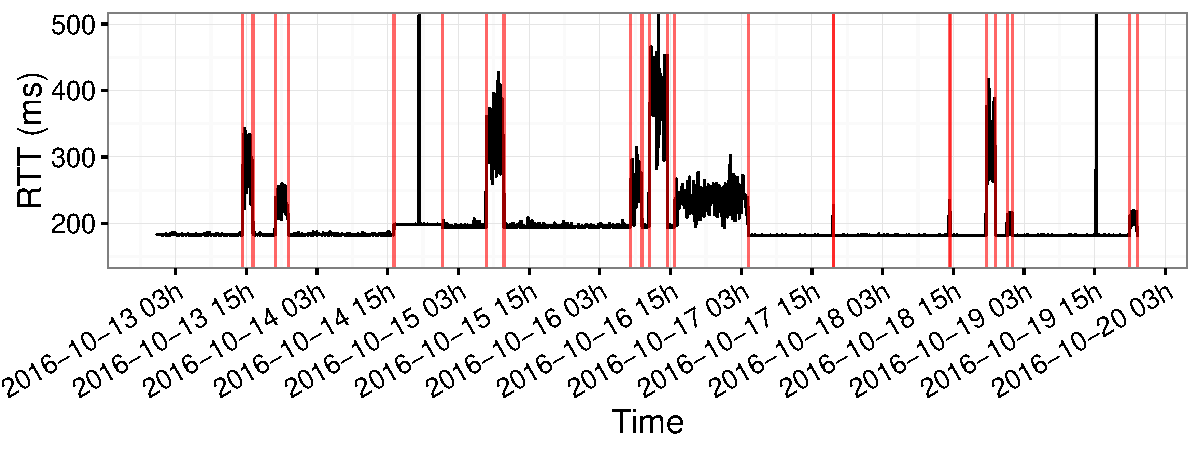
\includegraphics[width=.96\textwidth]{gfx/chap4/artificial_trace.pdf}
\caption{First 2500 %(out of 6506) 
Datapoints of an artificial RTT time series (one datapoint every 4min). 
Red vertical lines correspond to generated changes.}
\label{fig:art_example}
\end{figure}

In order to determine which detection method works the best on RTT time series, 
a dataset with \textit{a priori} labelled moments of RTT change is required, serving as ground truth, in the above presented scoring method. It's quality is essential to the relevance of evaluation results.

There are two approaches to a labelled ground truth: 1) artificially generated data; 2) real data with labels.
Real data is naturally the preferred choice and 
can only be labelled by humans with domain knowledge in absence of systematic automation, which is however tedious and error-prone. 
%Moreover, identifying significant change in RTT time series lacks an operational standard.
Therefore, it is of importance to first design tools facilitating the labelling and second to evaluate the quality of so produced `ground truth'.
More specifically, 1) a set of tools for interactive visual inspection (for RTT time series and labels) are developed to minimize human errors~\footnote{\url{https://github.com/WenqinSHAO/rtt_visual.git}}; 2) we fabricated a synthetic RTT dataset with known moments of actual change, and compared the human detection results to generated change moments~\footnote{\url{https://github.com/WenqinSHAO/rtt_gen.git}}. The labellers are the authors of this work, who are researchers/graduate students in networking. 
%JLR: we need to gain space. Delete.
%They were required to mark moments of RTT change worthy of inspection, according to their expertise and experience in the domain. %(no other guidelines were given apart from that).

The synthetic dataset contains 20 RTT timeseries %with 6485 datapoints on average,
representing 8646 hours of RTT measurements with 935 generated changepoints.
%The time interval between datapoints is 4min, in line with RIPE Atlas built-in ping measurement.
An example of these synthetic RTT trace is shown in Fig.~\ref{fig:art_example}.
Each trace contains several stages of random RTT level representing different underlying paths.
Each path has its own Markov process deciding the chance of getting into/out of a congestion phase. 
%The amplitude of each congestion segment is as well randomly generated.

\begin{figure}[!htb]
\centering
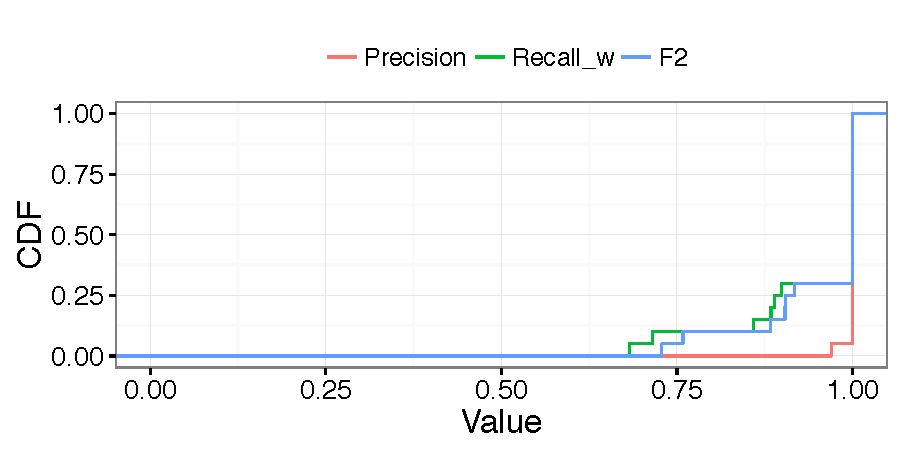
\includegraphics[width=.72\textwidth]{gfx/chap4/antoine_eval.pdf}
\caption{$Presicion$, $Recall_W$ and weighted $F_2$ of human labellers on synthetic dataset.}
\label{fig:antoine_eval}
\end{figure}
The detection performance of human labellers on the synthetic dataset is shown in Fig.~\ref{fig:antoine_eval}~\footnote{Note that the labellers had no idea these series were synthetic, since they are mixed up with real traces during labelling.}. 
Human labellers have $100\%$ for both $Precision$ and $Recall$ on 14 traces.
For the rest, the $Precision$ remains high. A few changes are miss out, but their total weight remain limited.

%Ensured that human labellers are capable of detecting changes, we proceed with real RTT traces. 
Real RTT traces of various characters are selected from RIPE Atlas to construct the ground truth dataset. Some are full of fluctuations; some contain periodic congestion, some have many stage changes, etc.
The entire dataset represents more than 34,008 hours, i.e. 1417 days, of RTT measurements. 1047 changepoints were identified by the labellers.
The labelled RTT traces along with the synthetic traces are all available in the main project repository given in Sec.~\ref{sec:cpt_data}.

\subsection{Candidate changepoint methods}
\label{sec:method}
According to the primer on changepoint detection in Sec.~\ref{sec:cpt}, there are two major parameters for a changepoint method formulated in that way: penalty and cost function/distribution.

We consider all the information criterion introduced (AIC, BIC, MBIC and Hannan-Quinn), and all the supported distribution types, including the non-parametric approach based on empirical distribution.

With some preliminary tests, we quickly realized that detection with Normal distribution tend to be over-sensitive, while Poisson, Exponential distribution are too numb.
It is because the mean and variance of Normal distribution are independently controlled by two parameters, which increases the chance of fitting subtle changes either in level or volatility.
Meanwhile, the mean and variance of Poisson and Exponential distribution are coupled by one parameter,
which restrains their freedom of adjustment~\footnote{Poisson, mean=variance=$\lambda$; Exponential, mean/variance=$\lambda$, mean=$1/\lambda$.}~\footnote{Gamma, mean/variance=$\beta$, mean=$\alpha/\beta$. \cite{Killick2013a} requires \textit{a priori} input for $\alpha$, which decides overall sensitivity. Therefore, only $\beta$ is tuned in finding changepoints.
%Larger $\alpha$ leads to more sensitive detection, as larger $\beta$ (smaller variance) will be resulted in fitting to a trace of certain mean value.
%The default option sets $\alpha$ set to 1, which degenerates the Gamma distribution to Exponential distribution. 
We tried $\alpha$ from 1 to 100 on the labelled dataset. None of them outperforms the best setting shown later on. Due to space limit, we no longer consider Gamma distributions.}.
For instance, for a path including trans-Pacific links, we shall expect a minimum RTT above 80ms, in which case the corresponding Poisson distribution could easily tolerate several RTT deviations of 20ms, which is already non-negligible.

%However, having coupled mean and variance is actually a desired feature. 
%We observed during labelling that the level of RTT and its variance are somehow positively related, particularly during congestion. 

To boost the detection sensitivity with Poisson and Exponential distribution, we propose a \textit{data transformation}: subtracting the RTT time series by its minimum value (baseline) to lower down its overall RTT level~\footnote{Note that timeout measurements are set to 1000ms. For Poisson distributions, RTT values are rounded to the closest integer.}. 
Changes are then detected for the baseline-removed RTT time series when assuming Poisson and Exponential distribution.
Such setting is denoted as \texttt{cpt\_poisson} and \texttt{cpt\_exp} respectively.
For the sake of comparison, we also consider Poisson distribution without data transformation and denote it as \texttt{cpt\_poisson\_naive.}
Normal distribution and non-parametric approach are applied directly on initial RTT measurements.
%\footnote{The data transformation is useless for these two methods.}.
%results uniform level shift over all potential segments in parameter estimation for Normal and non-parametric approach, thus pointless.}.
%% No need to explain why? OK
%%% Well, since I don't understand the explanation, better not... ;-))))))
They are denoted as \texttt{cpt\_normal} and \texttt{cpt\_np} accordingly.

\subsection{Evaluation of candidate methods}
\label{sec:eval}

Before evaluating with the scores defined in Sec.~\ref{sec:score}, one might wonder whether the RTT segments labelled by human beings already (Sec.~\ref{sec:label}) follow principally a specific distribution, and whether that distribution leads to the best detection performance.
We performed distribution test for 813 RTT segments longer than 20 datapoints against each of the discussed distribution types under corresponding data transformation (Sec.~\ref{sec:method}). 71 follow Normal distribution, 13 follow Poisson distribution, 
11 follow Exponential distribution~\footnote{Significance level 0.05. Shapiro-Wilk Normality test; %for Normal distribution
Chi-squared test for Poisson; Kolmogorov-Smirnov test for Exponential. Distribution parameters are estimated through Maximum Likelihood Estimation.}. None of these distributions seems to to have dominant popularity among the labelled RTT segments.

Changes are detected for selected real RTT traces with all distribution types.
The detection performance in terms of $Precision$, $Recall$, $Recall_W$, $F_2$ and weighted $F_2$ under optimal penalty are given in Fig.~\ref{fig:real_eval}.
More than $75\%$ of changes in terms of weight can be detected for more than half of the traces with any distribution.
All distribution types have better score in terms of recall and $F_2$ with their weighted variation, indicating some changepoints missed out are indeed of little operational importance.
Normal distribution has more fitting RTT segments than others, however its overall $F_2$ score (weighted or not) is not outstanding. This suggests that the goodness of fit is not a guarantee for detection performance.

Fig.~\ref{fig:real_eval} confirms that the detection with Normal distribution is over-sensitive even with MBIC, the largest adaptive penalty setting. For the other methods, their performances are rather close. 
\texttt{cpt\_poisson} seems to have a slight advantage according to weighted $F_2$.
Compared to \texttt{cpt\_poisson\_naive}, \texttt{cpt\_poisson} achieves higher $Recall_W$ without obviously sacrificing $Precision$.
As a matter of fact, without data transformation, assuming Exponential distribution detects no changepoint for a big part traces in the real RTT dataset.
These imply that the proposed data transformation has the potential to improve detection performance for these distributions. 

\begin{landscape}
\begin{figure}[!ht]
\centering
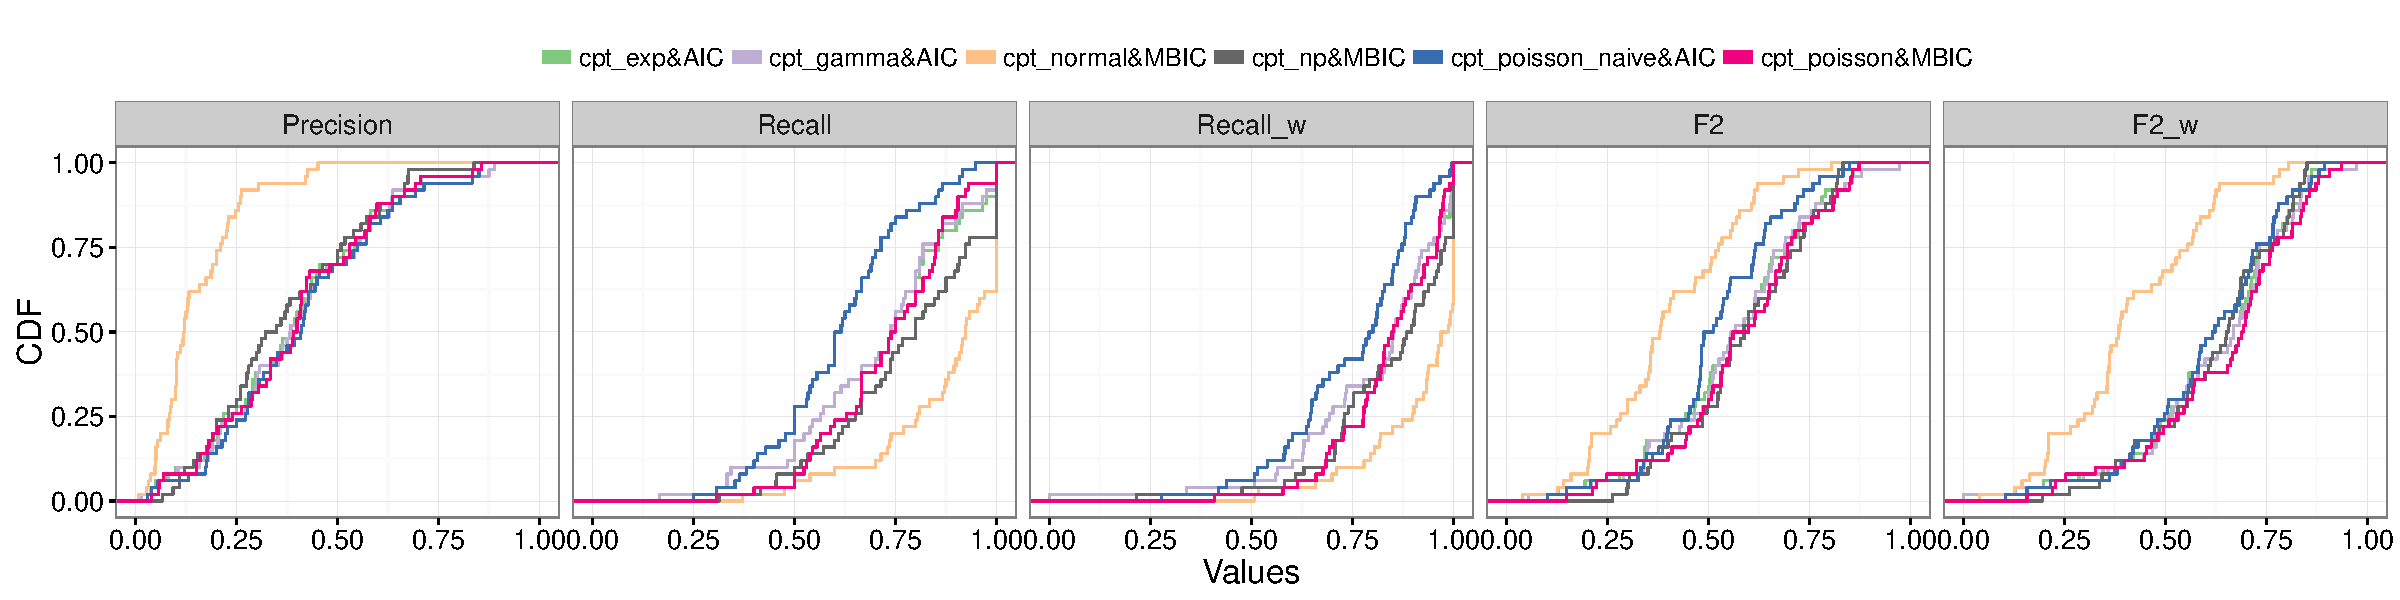
\includegraphics[width=1.8\textwidth]{gfx/chap4/real_eval_bis.pdf}
\caption{$Precision$, $Recall$, $Recall_W$, $F_2$ and $F_2W$ with weighted recall on real RTT traces.}
\label{fig:real_eval}
\end{figure}
\end{landscape}

\subsection{Characters of detected RTT changes}
\label{sec:cpt_trace}
\texttt{cpt\_poisson} and \texttt{cpt\_np} with MBIC are used to detected RTT changes for all the 6029 collected ping measurements.
We consider \texttt{cpt\_poisson} as it is the best performing one, though by a small margin.
\texttt{cpt\_np} is included as it performs well and its cost function follows a different principle.
%%% Well... It has also good performance right. Other wise you would not consider it...
%%% Yes, but rather close with the rest. Actually except normal, all the rest are rather close... so the reason choosing it instead of exponential is because the construction of cost function is fundamentally different.

%Since there is no guarantee that the traces included in labelled dataset covers all possible RTT morphology, it is thus possible that methods performs less well on evaluation dataset detects changepoints more appropriately on a larger dataset with richer characters.

\begin{figure}[!htb]
    \centering
    \begin{subfigure}[b]{.48\textwidth}
	\centering
	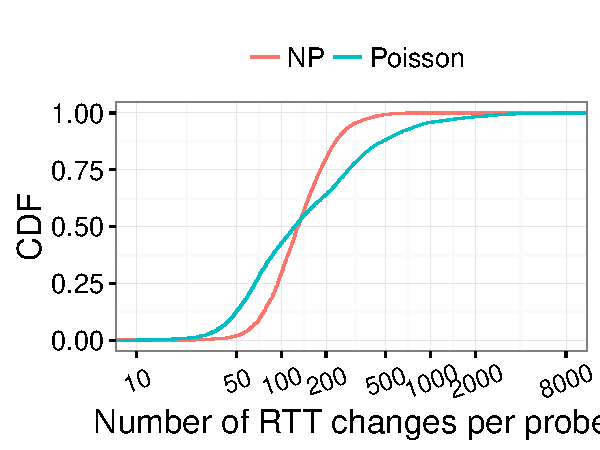
\includegraphics[width=\textwidth]{gfx/chap4/rtt_ch_count_cdf_cmp.pdf}
	\caption{\footnotesize CDF.}
	\label{fig:rtt_ch_count_cdf_cmp}
	\end{subfigure}
	\begin{subfigure}[b]{.48\textwidth}
	\centering
	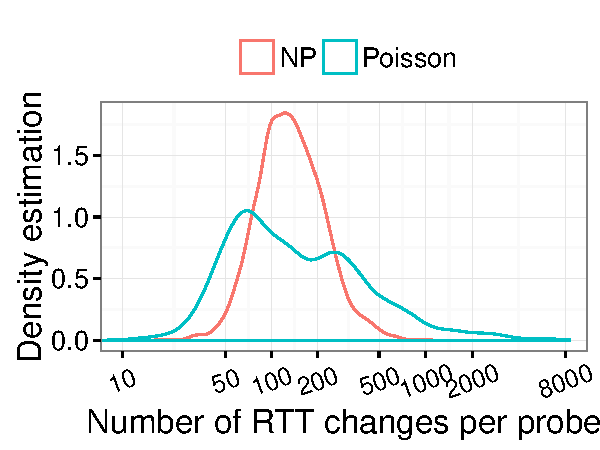
\includegraphics[width=\textwidth]{gfx/chap4/rtt_ch_count_density_cmp.pdf}
	\caption{\footnotesize Density.}
	\label{fig:rtt_ch_count_density_cmp}
	\end{subfigure}
\caption{RTT changepoints number distribution with different detection methods under MBIC.}
\label{fig:rtt_ch_count_cmp}
\end{figure}

Fig.~\ref{fig:rtt_ch_count_cmp} shows the distribution of RTT change numbers per probe. 4844 probe traces each containing more than 30,000 ping measurements are considered. 
854,626 RTT change are detected by \texttt{cpt\_np}.
\texttt{cpt\_poisson} almost doubled this number with 1,638,858 RTT changes.
However, the median change numbers for both methods is however the same (122).
Fig.~\ref{fig:rtt_ch_count_density_cmp} shows that the change number by \texttt{cpt\_poisson} spreads over a much wider range.
With \texttt{cpt\_poisson}, 711 probes ($11.86\%$) have more than 500 changes, while only 35 probes ($0.58\%$) with \texttt{cpt\_np} experienced that many changes.
This is probably because the cost function of \texttt{cpt\_np} bases on the estimation of quantiles (by default 10 quantiles used, more can be set) of empirical distribution. The dimension of $\theta$ is much larger than Poisson and Normal distribution. The penalty value increases hence much faster for \texttt{cpt\_np} when new changepoint is added, which prevents extremely large number of changepoints per probe trace.

\begin{figure}[!thb]
\centering
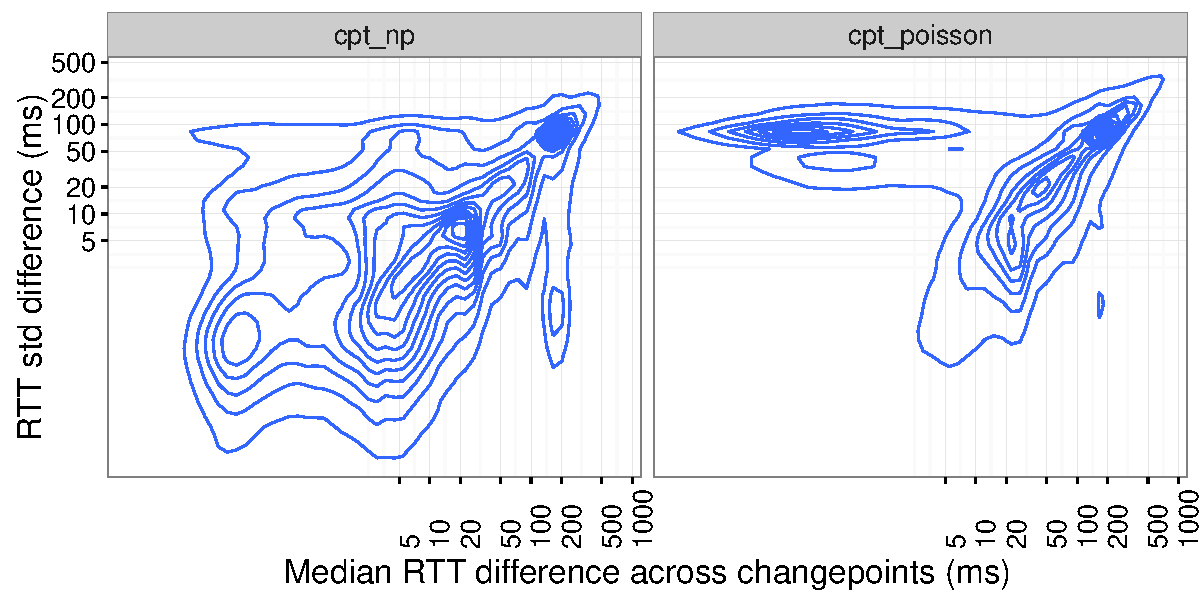
\includegraphics[width=.96\textwidth]{gfx/chap4/rtt_ch_chara_cmp.pdf}
\caption{Density estimation of RTT changepoints characteristics.}
\label{fig:rtt_chara_cmp}
\end{figure}
Fig.~\ref{fig:rtt_chara_cmp} compares the characters of all the RTT changes detected by the two methods.
Each RTT change is described by the associated level and volatility difference, i.e. $M$ and $\Delta$ defined in Sec.~\ref{sec:score}. 
Overall, RTT changes detected by \texttt{cpt\_poisson} are of larger $M$ and $\Delta$.
331,062 ($38.71\%$) changes with $M$ and $\Delta$ both smaller than 5ms are detected by \texttt{cpt\_np}.
With \texttt{cpt\_poisson}, there are only 87,021 ($5.31\%$) such changes of few importance in networking.
Meanwhile, a relatively bigger fraction of RTT changes detected by \texttt{cpt\_poisson} have large $\Delta$ but small $M$, more precisely 319,541 ($19.49\%$) with $M<5ms, \Delta>50ms$.
They are mostly associated with short RTT segments caused by frequent timeouts in certain probe traces. For example, probe 20854 had 2308 timeout measurements dispersed in the entire trace.
\texttt{cpt\_poisson} appears to be more sensitive to such sporadic but short living deviations.

%\spacedallcaps{Wrap-up} In this part, we described an evaluation framework adapted to change detection on RTT time series.
%A data transformation to improve the detection sensitivity is proposed,
%with which, Poisson distribution + MBIC achieves the most appropriate balance between sensitivity and relevance. The nuance between \texttt{cpt\_np} and \texttt{cpt\_poisson} will be further discussed in Sec~\ref{sec:corr}.

\section{Detecting path changes}
\label{sec:path}

In this section, we detect path changes experienced by collected RTT measurements, in order to explore in depth the detection sensitivity difference with different parameters and the detection relevance compared to path changes, network events known to have consequence on RTT.
Therefore, the purpose is not to repeat some of the studies sumeraized in~\ref{sec:rtt_path}, such as which kind of path change contributes most to RTT change, but rather to enhance the understanding on changepoint detection for RTT measurements.


\subsection{Routing change and \acf{LB}}

Among previous works summarized in~\ref{sec:rtt_path}, the contribution from IP-level LB to RTT variation is not clearly separated from those of real routing changes.
Schwartz et al.~\cite{Schwartz2010} regarded all paths between a source-destination pair as ``parallel paths'' and found out that RTTs over these paths were mostly overlapping.
However, there are two kinds of transitions among ``parallel paths'' that need to be distinguished.
They are 1) IP path changes caused by protocol level route recalculation, e.g. routing change after link failure or configuration update, 
and 2) those caused by LB mechanisms. 
Intra-domain path changes before the era of LB haven been shown to be responsible for important RTT changes~\cite{Pucha2007}. 
On the other hand, LB paths are of equal/close administrative cost, hence similar characteristics~\cite{Augustin2011}.
 
Trivial as it may sound, detecting IP path changes is challenging for RIPE Atlas built-in traceroute measurements.
The difficulties come from two aspects: 1) the wide deployment of IP-level LB; 2) RIPE Atlas uses Paris traceroute with different Paris IDs every other measurement (incremented by 1, recycling between 0 and 15)~\cite{Augustin2006, Pelsser2013}.

IP paths taken by two neighbouring measurements can naturally differ -- 
load-balanced on different available paths.  
From this angle, plain IP path changes doesn't mean that there were topological or configuration changes that lead to any real routing change. 
On the other hand, having different Paris IDs every time can also be helpful in this context.  If traceroute were locked on a single Paris ID, it would then be impossible to detect routing changes that only affect paths corresponding to other Paris IDs.

\subsection{IP Forwarding Pattern change}
When a different IP path is measured with a same Paris ID,
there is potentially a routing change. We call this kind of IP path change an \ac{IFP} change.
In the example below, the IFP change happens when Paris ID 2 begins to take IP path E instead of B. We refer to two measurements with same Paris ID but different IP paths as \textit{conflicting} measurements.
\begin{Verbatim}[fontsize=\small]
                             | IFP change
Paris ID: 0 1 2 3 4 .. 15 0 1|2 3 ..
IP Path:  A B B A A .. C  A B|E E ..
       A measurement series  | boundary -> forward
\end{Verbatim}

IFP changes can thus be identified by constructing a set of measurement series, each containing no conflicting measurements. Yet, across two series next to each other, there shall be as least one pair of conflicting measurements, otherwise they can be merged.
This can be done by moving the boundary of measurement series \textit{forward} to include non-conflicting measurements, till a conflict is encountered, as shown in the above example.
We call this approach \textit{forward inclusion}.

The drawback of \textit{forward inclusion} is that it potentially delays the detection of actual IFP changes.
This is because, when including non-conflicting measurements forwardly, a measurement series always has the chance to absorb measurements till it experiences all possible Paris IDs.
However an actual IFP change could happen before that moment.
An example of possibly delayed IFP change is given right below:
\begin{Verbatim}[fontsize=\small]
        !Possible position of actual IFP change        
.. 1|2 3!4 5 .. 15 0 1|2 3 4 5 ... 15 0 1 2 3 4 5 ..
.. B|B A!A C .. C  A B|E E A C ... C  A B E E A C ..
                      | IFP change forward inclusion
                      | backward <- boundary
\end{Verbatim}
With \textit{forward inclusion}, an IFP change will be detected at the 2nd appearance of Paris ID 2.
While the actual change probably happens at the 1st appearance of Paris ID 4, since starting from it, all the measurements are non-conflicting with the later measurement series.
The 1st appearance of Paris 2 and 3 are in fact a short deviation from a popular IFP.

Cases like this are highly possible, because networks tend to have some stable configurations that lead to a few dominant paths over time~\cite{Chandrasekaran, Pucha2007}. 
Deviations from dominant/popular IFPs are thus likely to be short living.
With RIPE Altas built-in measurements, they probably won't last long enough to experience all the Paris IDs~\footnote{It takes at least 450min (30min * 15) to go through all the 16 Paris IDs used in RIPE Atlas built-in traceroute.}.
To maximize the presence of popular IFPs, we only push backwardly the boundary obtained by \textit{forward inclusion} if 1) the latter measurement series is longer than the previous one; 2) the latter measurement series experiences all the Paris IDs at least twice.
We refer to this approach as \textit{backward extension}.
We show later on that IFP changes detected by \textit{backward extension} have a much larger chance matching with RTT changes.

\subsection{Characters of detected path changes}
AS-level path changes are as well detected after translating IP hops to ASN hops~\cite{routeviews}.
We didn't consider third-party address~\cite{Hyun2003, Zhang2010} and IP alias techniques\cite{Gunes2009,Keys2010a} in this operation.
It is because the focus is to detect changes instead of constructing an accurate Internet topology.
We did detect the presence of IXPs using the heuristics proposed by traIXroute~\cite{Nomikos2016}, since individual studies have shown that IXP could be involved in large RTT changes~\cite{kopp2016}.

\begin{figure}[!htb]
    \centering
    \begin{subfigure}[b]{.48\textwidth}
	\centering
	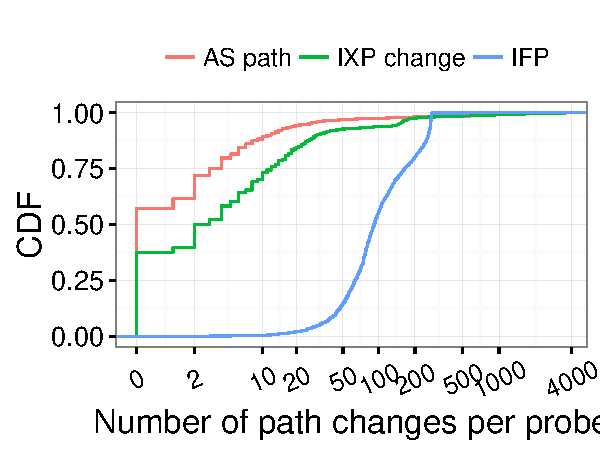
\includegraphics[width=\textwidth]{gfx/chap4/path_ch_count_cdf_cmp.pdf}
	\caption{\footnotesize CDF.}
	\label{fig:path_ch_count_cdf_cmp}
	\end{subfigure}
	\begin{subfigure}[b]{.48\textwidth}
	\centering
	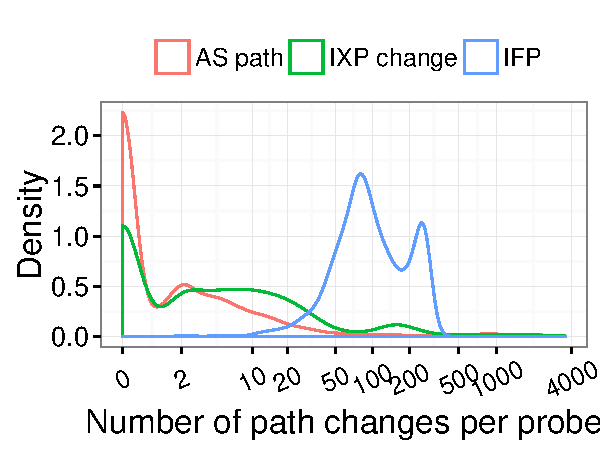
\includegraphics[width=\textwidth]{gfx/chap4/path_ch_count_density_cmp.pdf}
	\caption{\footnotesize Density.}
	\label{fig:path_ch_count_density_cmp}
	\end{subfigure}
\caption{Path change times per probe trace distribution. One probe with most complete traceroute measurement is chosen for each AS. 2050 probes/ASes are inlcuded in the graph.}
\label{fig:path_ch_count_cmp}
\end{figure}
We consider only AS path changes where the difference starts from a hop position involving public ASNs in both AS paths.
Difference due to temporal presence of non-responding hops are ignored.
IXP change happens when the difference starts from a position involving at least one IXP hop in the two AS paths.
IFP changes, detected with \textit{backward extension}, not overlapped with AS path/IXP changes are considered.
They are potentially caused by intra-domain routing changes.

The distribution of number of path changes per probe trace
is illustrated in Fig.~\ref{fig:path_ch_count_cmp}.
One probe with the most complete traceroute measurements is selected for each of the 2050 source ASes.
1170 ($57.07\%$) of them experienced no AS path changes over the period of three months, indicating that the AS paths are in general very stable over time.
Still, 51 ($2.49\%$) probes underwent more than 100 AS path changes.
717 probes ($34.98\%$) didn't have any IXP change.
140 probes experienced frequent ($> 100$) IXP changes.
IFP changes are much more frequent than the other two path changes. 
Half of the selected probes experienced more than 90 IFP changes.
We investigate the nature of these path changes, together with their potential impact on RTT, in Sec.~\ref{sec:corr}.

\section{Match between RTT and path changes}
\label{sec:corr}

If a pair of RTT and path change are close in time, chances are that the RTT changes is caused by the path change. We say that these two changes are correlated. This is a demonstration of relevance between detected RTT change and underlying routing activities.
%We are interested in knowing the fraction/quantity of RTT and path changes that

However, there is no straightforward matching between the two changes, as the measurement intervals are different: $30min$ for traceroute while $4min$ for ping. 
Again, \textit{minimum cost maximum-cardinality matching} appears to be a reasonable formulation of the correlation between RTT and path changes.
We therefore borrow the concept of optimal matching in changepoint evaluation (Sec.~\ref{sec:score}).
The shift tolerance window is set to the interval of traceroute measurement, as causal relationship between the RTT and path change is possible within that range.
A pair of RTT and path changes are correlated/matched if they are within in the so produced optimal matching.
The notion $Precision$, introduced in section~\ref{sec:score}, is now interpreted as the fraction of path changes that are matched to an RTT change. 

\begin{figure}[!htb]
\centering
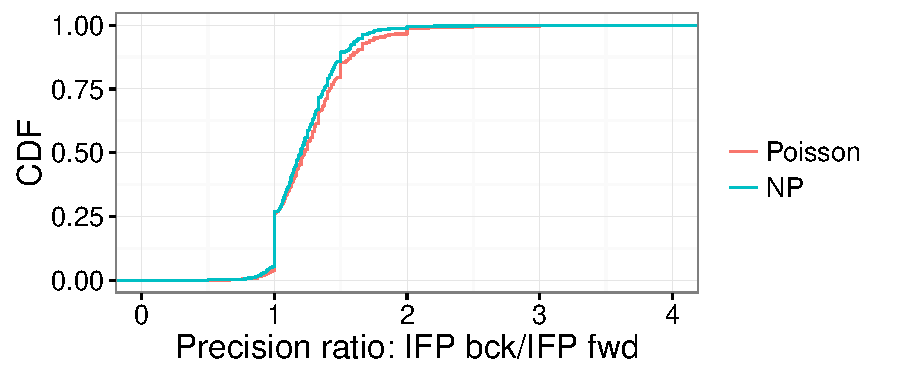
\includegraphics[width=.72\textwidth]{gfx/chap4/ifp_bck_ch_precision_gain_cdf.pdf}
\caption{Precision ration between IFP changes detected by \textit{backward extension} and \textit{forward inclusion}.}
\label{fig:ifp_bck_ch_precision_gain_cdf}
\end{figure}
Fig.~\ref{fig:ifp_bck_ch_precision_gain_cdf} shows that with same number of changes, IFP changes detected with \textit{backward extension} are much more likely to have a match with RTT changes for $75\%$ probes.
The significant increase in precision implies the occurrences of short IFP deviations, as well confirms the success of \textit{backward extension} in capturing them.

\begin{table}[!htb]
\caption{Number of RTT changes matched with a path change for the selected 2050 probes.}
\label{tab:corr_overview}
\centering
\footnotesize
\setlength{\tabcolsep}{0.5em}
\begin{tabular}{l|cc|c}
\toprule
& \texttt{cpt\_poisson} & \texttt{cpt\_np} & \# path changes\\
\midrule
AS path change & 11,794 & 6,380 & 51,282 \\
IXP change & 9,126 & 8,341 & 73,544\\
IFP change & 38,700 & 36,400 & 244,713\\
\midrule
\# RTT changes & 481,877 & 307,312 & \\
\bottomrule
\end{tabular}
\end{table}

Tab.~\ref{tab:corr_overview} details the number of matched RTT and path change pairs.
A large fraction of path changes doesn't match with any RTT changes.
Especially, the fraction of AS path changes matched to RTT changes with either detection method is much lower than the reported $72.5\%$ in \cite{Rimondini2014}.
An important part of RTT changes detected by both method doesn't match with any change in the forwarding path either.
Moreover, the number of RTT changes correlates with AS path changes differs greatly across the two changepoint methods,
while the number matched to IXP or IFP change are relatively close.
We explore the underlying reasons behind above phenomena.

\section{Change detection sensitivity and relevance}
\subsection{\texttt{cpt\_poisson} matches better with AS path change?}
\label{sec:as_match_diff}
Among 880 probes ever experienced AS path changes, 293 probes have more AS path changes matched to \texttt{cpt\_poisson} RTT changes, 224 have more AS path changes matched to \texttt{cpt\_np} changes, 
Among these 517 probes, 463 are with a difference smaller than 10 changes.
The rest 363 probes have no difference across the two methods.
Contrary to what we see in Tab.~\ref{tab:corr_overview}, the numbers of AS path matched are in fact highly consistent across the two methods for the majority of probes.
The difference is caused by a small fraction of probes identified in Fig.~\ref{fig:as_match_diff}
More the color (of a probe) is on the red side, more important the difference is between \texttt{cpt\_poisson} and \texttt{cpt\_np}.
We can tell that those probes plainly in red all experienced a large number of AS path changes (y-axis).
Moreover, if more path changes are matched to RTT changes detected by one method, very likely more RTT changes are as well detected by this method than the other.
All together, the difference in matched RTT changes with AS path changes fundamentally lies in the difference of detection sensitivity (number of detected RTT changes) across different probe traces. This difference is manifested through extremely frequent AS Path changes of several specific probes.

\begin{figure}[!htb]
\centering
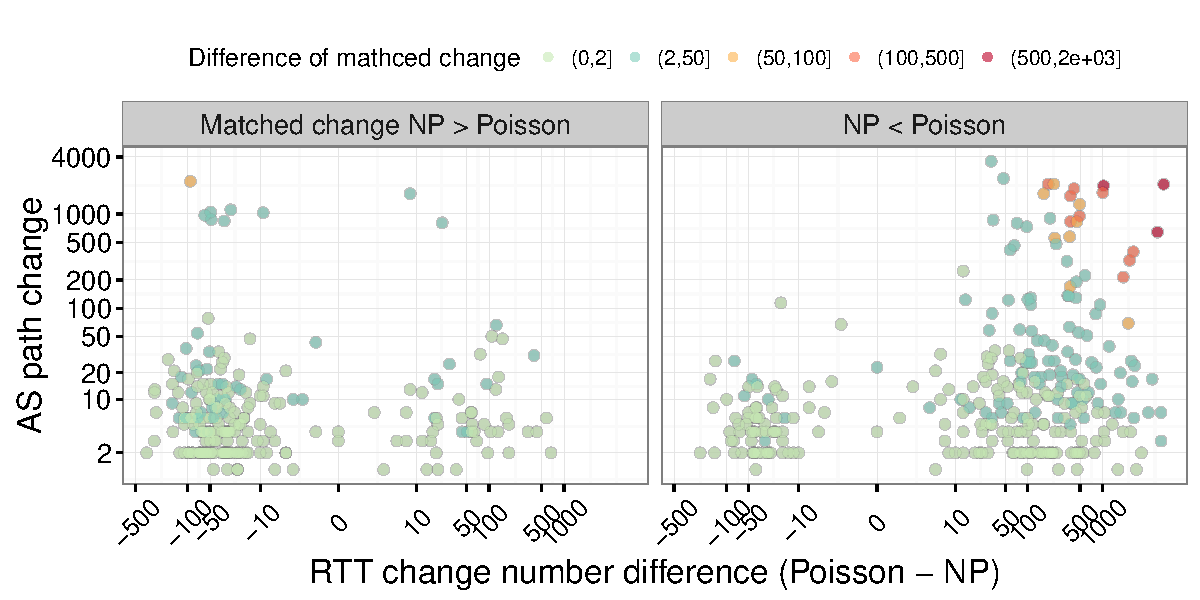
\includegraphics[width=.96\textwidth]{gfx/chap4/as_match_diff.pdf}
\caption{Probe having difference in the number of AS path changes matched to RTT changes detected by \texttt{cpt\_poisson} and \texttt{cpt\_np}. Probes are characterized by its AS path change numbers and RTT change number difference between the two methods. The color of each probe indicates the level of difference in matched change. Left panel shows the probes with more AS path changes matched to \texttt{cpt\_np} RTT changes.}
\label{fig:as_match_diff}
\end{figure}

\begin{figure}[!htb]
\centering
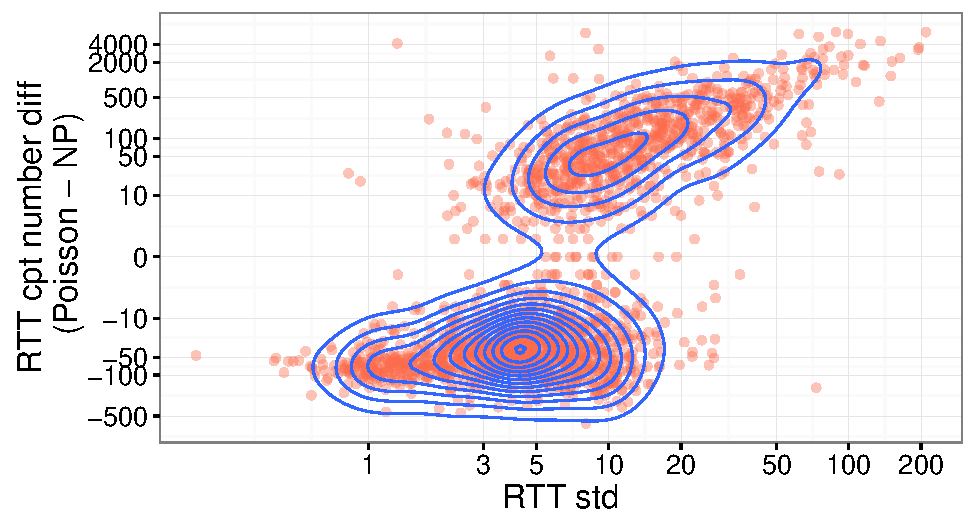
\includegraphics[width=.64\textwidth]{gfx/chap4/cpt_diff_vs_std.pdf}
\caption{Relation between RTT change number difference by the two changepoint method and the RTT trace $std$.}
\label{fig:cpt_diff_vs_std}
\end{figure}

Fig.~\ref{fig:rtt_ch_count_density_cmp} and Tab.~\ref{tab:corr_overview} already tell that \texttt{cpt\_poisson} detects in total more RTT changes than \texttt{cpt\_np}, appearing to be more sensitive.
However, for most probes with small overall RTT variation, \texttt{cpt\_np} is in fact more sensitive and detects more RTT changes, according to Fig.~\ref{fig:cpt_diff_vs_std}.
This matches with Fig.~\ref{fig:rtt_ch_count_density_cmp} in the sense that \texttt{cpt\_np} detects much more changes of small amplitude.
For probes with relatively large overall RTT variation, \texttt{cpt\_poisson} tends to be more sensitive and the difference in change number increases with the level of RTT variance.
With comprehensive manual inspection, we found that those RTT traces with high variance mostly underwent large amplitude RTT oscillations, many of which caused by ping timeouts. As human change detector, we also found very difficult to mark moments of change for these traces.

\subsection{How AS path changes match to RTT changes?}
\begin{figure}[!htb]
    \centering
    \begin{subfigure}[b]{.48\textwidth}
	\centering
	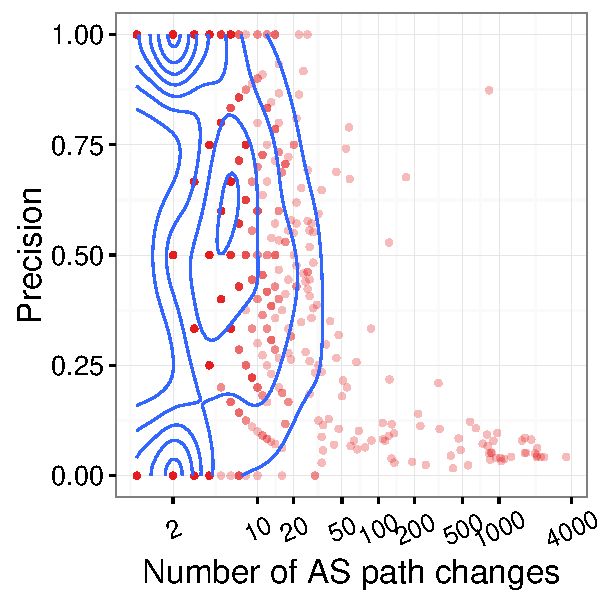
\includegraphics[width=\textwidth]{gfx/chap4/as_path_ch_precision_np.pdf}
	\caption{\footnotesize changes by \texttt{cpt\_np}.}
	\label{fig:as_path_ch_precision_np}
	\end{subfigure}
	\begin{subfigure}[b]{.48\textwidth}
	\centering
    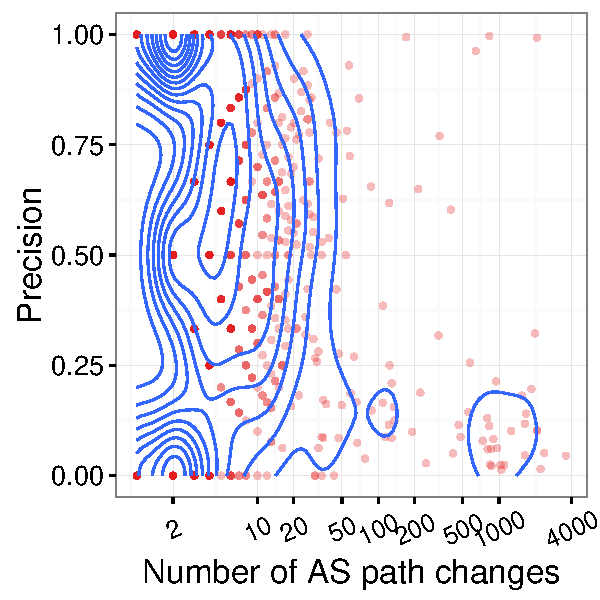
\includegraphics[width=\textwidth]{gfx/chap4/as_path_ch_precision_poisson.pdf}
	\caption{\footnotesize changes by \texttt{cpt\_poisson}.}
	\label{fig:as_path_ch_precision_poisson}
	\end{subfigure}
\caption{The relation between precision and AS path change times per probe trace.}
\label{fig:as_path_ch_precision}
\end{figure}

\begin{figure}[!htb]
\centering
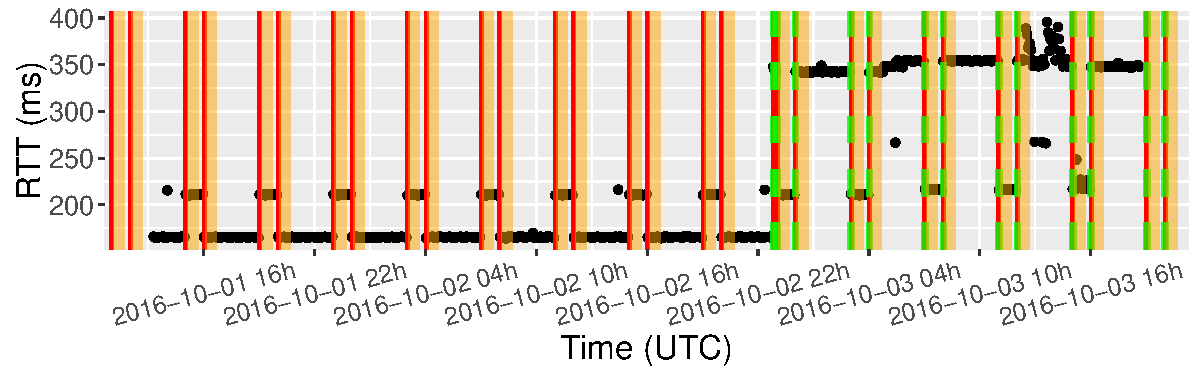
\includegraphics[width=.96\textwidth]{gfx/chap4/case_12849.pdf}
\caption{RTT from Probe 12849. Red lines for RTT change detected by \texttt{cpt\_poisson}; green dotted lines for RTT change by \texttt{cpt\_np}. Orange strips for AS path changes.}
\label{fig:case_12849_rtt}
\end{figure}
A nature question following the above analysis is whether those frequent AS path changes can in fact cause RTT changes.
Fig.~\ref{fig:as_path_ch_precision} reveals that probes with extremely frequent AS path changes have in fact very low correlation, in terms of precision, with RTT changes.
After extensive manual inspection, those frequent AS path changes appear to be AS-level LB, i.e. upstream ASes in reaching the destination are switched very frequently among a few providers.
Such AS changes generally don't have a clear impact on the RTT level. 


Yet, not all such AS-level load balancing is without consequence. For example, probe 12849 in Fig.~\ref{fig:case_12849_rtt} experienced 170 AS path changes, among which 169 are matched to RTT changes detected by \texttt{cpt\_poisson} and only 102 are matched to \texttt{cpt\_np}.
These AS path changes are highly periodic and coincide with clear cut RTT changes.
\texttt{cpt\_np} failed to detect some of the changes with smaller amplitude.

\subsection{Pitfalls of IXP and IFP change detection}
Similar to AS path changes, the correlation with RTT changes is weak for frequent IXP and IFP changes.
In Fig.~\ref{fig:path_ch_count_density_cmp}, a group of probes are in the area of 100 to 200 IXP changes. Their correlation with RTT changes is fairly low, precision  around $0.1$.
We investigate all the 58 probes in the area. These probe passed by AMS-IX to reach b-root most of the time. There were about 147 times, shared by these probes, where AMS-IX hop was replaced by a timeout hop before arriving AS6939.
In such case, no IXP related address appears in the measured path. The presence of IXP is thus uncertain \footnote{The newly released traIXroute v2.1 can detect IXP without the presence of IXP related IP address, if the neighbouring ASes are known to be member of a same IXP. However, it is still possible that two ASes peer at multiple IXPs, where the exact IXP traversed would remain uncertain.}.

\begin{table}[!htb]
\caption{Quantiles of IP path numbers per probe trace.}
\label{tab:ip_path_count}
\centering
\footnotesize
\setlength{\tabcolsep}{0.5em}
\begin{tabular}{ccccccc}
\toprule
$5\%$ & $10\%$ & $25\%$ & $50\%$ & $75\%$ & $95\%$ & $100\%$\\
\midrule
20 & 32 & 56 & 91 & 145 & 419 & 4302\\
\bottomrule
\end{tabular}
\end{table}

The correlation of IFP changes with RTT changes are much weaker than that of AS and IXP path changes.
It turned out that most probes experienced much more than 16 end-to-end IP paths, Tab.~\ref{tab:ip_path_count}.
In such case, one Paris ID might have been mapped to more than one IP path in reality, which leads to IFP changes without actual routing change in the forward path.
Within in each single AS, the number of different IP paths rarely exceeds 16 toward a destination. However a chain of ASes can produce way much richer combinations of end-to-end IP paths.

Moreover, there is a group of probes having around 250 IFP changes according to Fig.~\ref{fig:path_ch_count_density_cmp}.
An IFP change takes place roughly every 16 measurements on these probes. 
These changes are as well poorly correlated to RTT changes.
%$250 \times 16 = 4000$ is about the total number of traceroute measurements over 3 months.
We investigated some probes in the area and found out the frequent changes aren't necessary related to the large amount of end-to-end paths.
For some probes, two neighbouring IFPs only differ at one or two Paris IDs.
IP paths taken by these Paris IDs oscillates between a few alternatives frequently.
For example, the Paris ID 6, 7, 8, 9 of probe 23998 switches a lot among only 2 paths.
Such change in general doesn't have obvious consequence on RTT level.

\subsection{Unmatched RTT changes}

\begin{figure}[!htb]
    \centering
    \begin{subfigure}[b]{.96\textwidth}
	\centering
	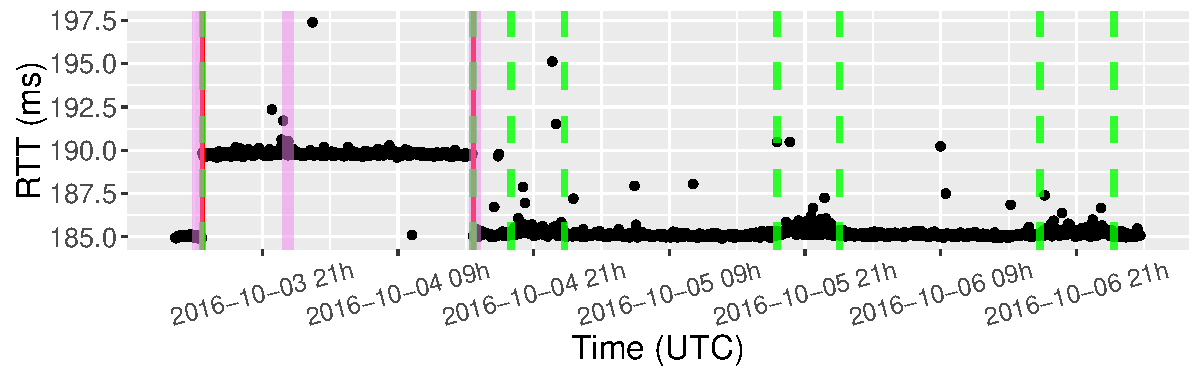
\includegraphics[width=\textwidth]{gfx/chap4/case_28002.pdf}
	\caption{\footnotesize Probe 28002.}
	\label{fig:case_28002}
	\end{subfigure}
	\begin{subfigure}[b]{.96\textwidth}
	\centering
	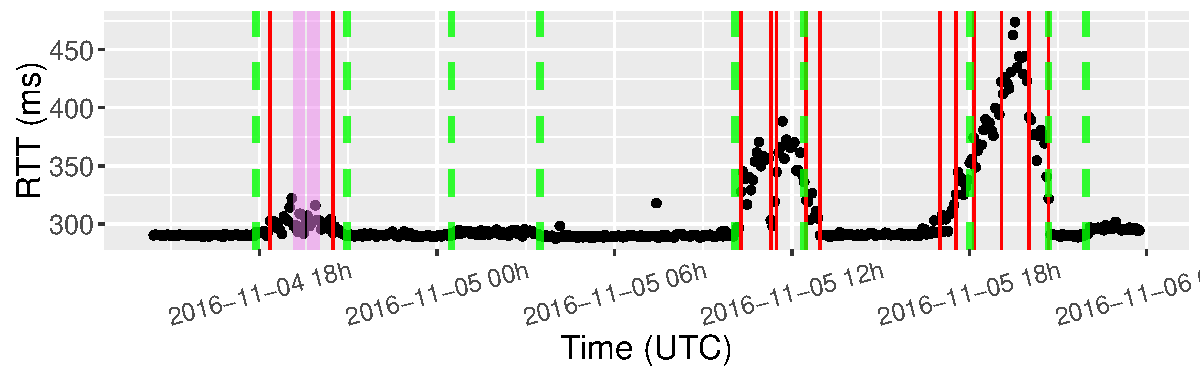
\includegraphics[width=\textwidth]{gfx/chap4/case_26328.pdf}
	\caption{\footnotesize Probe 26328.}
	\label{fig:case_26328}
	\end{subfigure}
\caption{RTT trace and change detection example. Red lines for RTT change detected by \texttt{cpt\_poisson}; green dotted lines for RTT change by \texttt{cpt\_np}. Violet strips are IFP changes.}
\label{fig:case_sensitivity}
\end{figure}

Several reasons contribute to the large amount and fraction of RTT changes unmatched to any path changes.
First, some path changes experienced by RTT measurements are not observed. We were not able to measure the reverse path with RIPE Atlas built-in measurement, let alone detecting the changes on the reverse path. However, these changes could have contributed to RTT changes, especially in the context of inter-domain routing where paths are likely to be asymmetric.
Second, congestion. Fig.~\ref{fig:case_26328} gives an typical example of RTT changes probably caused by congestion.
%as both RTT variance and level increase correspondingly. 
Congestion like this doesn't repeat periodically, and thus can not be detected with existing methods~\cite{Luckie2014}.
Changepoint methods studied in this work can be potentially employed to pinpoint such transient congestion and estimate their
impact on the tranmission performance. We envision it as future work.
If we boldly assume that path changes on reverse paths cause comparable amount of RTT changes as forwarding paths do, there are still many RTT change unmatched. Some of them might be effectively attributed to congestion.
Third, RTT change detection can be over-sensitive. We revealed from a macroscopic view in Sec.~\ref{sec:cpt_trace} and ~\ref{sec:as_match_diff} that \texttt{cpt\_poisson} tend to overestimate the number of changepoints when the RTT trace is noisy, while \texttt{cpt\_np} is capable of detecting delicate RTT changes. Individual traces are given in Fig.~\ref{fig:case_sensitivity} to illustrate the sensitivity difference from a microscopic view. In Fig.~\ref{fig:case_28002}, \texttt{cpt\_np} detected all the periodic small amplitude congestion. In Fig.~\ref{fig:case_26328}, both methods identified the two large `plumbs' near the end of the trace. The difference is that \texttt{cpt\_poisson} marked intermediate level changes as well.

\section*{Conclusion}
In this chapter, we proposed an evaluation framework for change detection on RTT time series.
The framework is robust with human-labelled dataset and weights RTT changes according to their importance in network operation. We further designed a data transformation adapted to RTT measurements to improve the detection sensitivity of some detection methods.
In detecting path changes, we distinguish those caused by routing changes from those due to load balancing.
Finally, we correlate the detected RTT and path changes by establishing an one-to-one matching between them. 
We investigated the sensitivity distinction across different change detection methods. 
Hidden issues with path changes are as well revealed.

This work is mere a facilitator for measurement-based TE. Further efforts are required in building a working system. To name a few: online detection of RTT changes, route selection logic triggered by change detection  etc.
